\documentclass{llncs}
\newcommand{\Section}[1]{\vspace{-8pt}\section{\hskip-1em.~~#1}\vspace{-3pt}}
\newcommand{\SubSection}[1]{\vspace{-3pt}\subsection{\hskip -1em.~~#1}\vspace{-3pt}}
\newcommand{\X}{{\bf X}}
\newcommand{\x}{{\bf x}}
\newcommand{\Y}{{\bf Y}}
\newcommand{\y}{{\bf y}}
\newcommand{\Z}{{\bf Z}}
\newcommand{\z}{{\bf z}}
\newcommand{\bs}{\boldsymbol}
\newcommand{\bSigma}{\boldsymbol \Sigma}
\usepackage{amsmath,amssymb,algorithm,algorithmic}
\usepackage{times}
\usepackage{setspace,verbatim}
\usepackage{epsfig,url}

\begin{document}
\vspace{-0.1in}
\title{Partial sparse canonical correlation analysis (PSCCA) for population
  studies in medical imaging}
\author{Anonymous}
\institute{Anonymous}
\maketitle              
%\vspace{-0.1in}
\begin{abstract}
We propose a new multivariate method, partial sparse canonical
correlation analysis (PSCCA), for computing the statistical
comparisons needed by population studies in medical imaging.  PSCCA is a
multivariate generalization of linear regression that allows one to statistically parameterize imaging studies in terms of
multiple views of the population (e.g., the full collection of
measurements taken from an image set along with batteries of cognitive
or genetic data) while controlling for nuisance variables.  This paper
develops the theory of PSCCA, provides an algorithm and illustrates
PSCCA performance on both simulated and real datasets.  We show that
PSCCA can improve detection power over standard univariate approaches
while retaining the interpretability and biological plausibility of
the estimated effects.  We also discuss the strengths, limitations and
future potential of this methodology.
\end{abstract}
%\vspace{-0.2in}
\section{Introduction}
% pubmed references to MRI :  
% 2000-2001 --- 25561
% 2001-2002 --- 27053
% 2003-2004 --- 31708
% 2005-2006 --- 38620
% 2008-2009 --- 49288
% 2009-2010 --- 49323
% pubmed references to MRI brain :  
% 2000-2001 --- 9938
% 2001-2002 --- 
% 2003-2004 --- 12655
% 2005-2006 --- 
% 2008-2009 --- 
% 2009-2010 --- 19676 ------  
% MRI brain statistical parametric mapping 783 results ,
% MRI brain gives 
The number of neuroimaging studies published annually has doubled from
9,938 in 2000-2001 to 19,676 in 2009-2010
(\url{http://www.ncbi.nlm.nih.gov/pubmed/}).  This growth has been
accompanied by increasing diversity in the types of data being
collected;  Imaging studies now often include not only various
structural and functional modalities but also neurocognitive
batteries, genetics, and environmental measurements.  However,
the statistical methods have changed relatively
little over the past twenty years -- until very recently
(e.g., \cite{Tosun2010a}).  The increasing size of imaging
datasets and the concomitant desire for performing integrative studies
across modalities points to the need for new multivariate statistical
methods that elegantly handle large, multi-view datasets while
retaining or even improving detection power over traditional
mass-univariate models such as statistical parametric mapping (SPM).

Canonical Correlation Analysis (CCA)~\cite{hotellingcca} is a
traditional multivariate generalization of standard linear regression
\cite{kshirsagar}.  CCA inherently avoids the multiple-comparisons
penalty associated with mass-univariate methods by symmetrically
maximizing the correlation between the full matrices representing two
views of the data (here denoted $\Y$ and $\X$).  The matrix {$\X$}
might represent a tabulation of all demographic data, including
genetics, diagnosis, behavioral measures, age, etc. while $\Y$ is a
matrix of all the imaging measurements.  In contrast, traditional
univariate models only enable the predicted value to be a vector while
the predictors may be a matrix.  In both traditional regression and CCA, the
number of predictors must be fewer than the number of observations.

Recently, sparse (or penalized) canonical covariance
analyses (SCCovA) ~\cite{parkhomenko,witten,lykou} have been proposed
as an approximation to CCA specifically for the high dimensional
($p\gg n$) setting where $n$ is the number of observations (subjects
in our neuroimaging study) and $p$ is the number of predictors (e.g. voxels
in the brain).\footnote{SCCovA substitutes the identity matrix for
within-view covariance matrices and thus analyze cross-covariance
structure, not correlation structure \cite{cherry}}  The {\em
sparseness} of penalized methods improves interpretability by including in the model
only the most important variables from the large set of $p$
predictors.  From a medical imaging researcher's perspective, the
benefit is that only parts of the brain that are most predictive will
emerge in the results provided by a penalized statistical tool.
Hence, brain regions are highlighted in a way that is similar to
SPM.  In contrast, however, regions selected by SCCovA (or similarly
sparse canonical correlation analysis (SCCA)) are treated
statistically as a collective (or `network') as opposed to as
independent variables.

Despite prior neuroimaging studies using SCCA \cite{Avants2010b}, we
are unaware of previous work which studies factoring (``partialling'')
out nuisance covariates with a penalized approach to CCA.  While this
problem has been addressed historically by partial canonical
correlation analysis (PCCA)\cite{timm}, no sparse formulation has yet been
proposed.  In this paper, we provide the theory required for Partial Sparse CCA
(PSCCA) and present a novel and efficient iterative algorithm for
PSCCA. As mentioned earlier, PSCCA (like CCA) performs a single global
multivariate test over the whole region of interest (e.g. all
voxels in the cortex). PSCCA identifies
the subset of the brain most associated with the variable(s) of interest
(for instance, a cognitive battery) while factoring out confounding
effects (age, gender).  Thus, PSCCA may be applied to almost any statistical
scenario in medical imaging studies traditionally handled by SPM.  
% It is not the ``parameter'' that find the subset

The rest of the paper is organized as follows: in the next section we
provide a brief review of CCA and Sparse CCA. In Section 3, we present
the theory behind Partial Sparse CCA (PSCCA) and describe our novel
iterative algorithm for performing PSCCA. In Section 4, we provide
experimental results on synthetic and real world neuroimaging datasets
and we conclude with a brief summary in Section 5.

%What we are doing here ( a few sentences )

%This paper will detail and illustrate our approach to performing
%neuroimaging studies in the style of traditional formulations but
%using a new, powerful multivariate pscca.  We highlight in both
%simulated and real data the advantages and disadvantages of this
%method.

%\vspace{-0.2in}

\section{Brief review: CCA and sparse CCA (SCCA)}
\begin{comment}{
Consider a standard neuroimaging population study with both male and
female subjects between 20 and 40 years of age each of which measured
via a series of MRI scans.  Each subject is also designated either
patient or control.  A standard regression analysis will treat the
quantitative imaging measurement as the dependent variable ($\y$) and
age, gender and diagnosis group as covariates $({\X})$ where each test
is performed independently at each voxel.  Detection power is
compromised by the multiple-comparisons problem incurred by the number
of imaging measurements (millions) as well as the confounding
variables (age, gender).  If we are using mass-univariate models and
want to test the whole brain for effects, then
we can not do much about the first problem.  For the second problem,
we can factor out the effects of these unwanted (confounding)
variables by regressing on the residuals ($\y -\X\beta$).
}
\end{comment}

CCA~\cite{hotellingcca} is the analog to Principal Component Analysis
(PCA) for pairs of matrices. PCA computes the directions of maximum
covariance between elements in a single matrix, whereas CCA computes
the directions of maximal correlation between a pair of matrices.
See~\cite{taylor:cca} for a general review of CCA along with some
representative applications.  %Unlike PCA, CCA does not depend on how
%the observations are scaled.

More specifically, given a set of $n$ paired observation vectors
$\{(y_1,x_1),...,(y_n,x_n)\}$--in our case the two matrices are the
quantitative imaging measurement ({\Y}) and age, gender, diagnosis ({\X}) matrices --we would like to simultaneously find the directions
${\bs{\bs\phi_{\Y}}}$ and
${\bs{\bs\phi_{\X}}}$ that maximize the correlation of
the projections of ${\Y}$ onto ${\bs{\bs\phi_{\Y}}}$
with the projections of ${\X}$ onto
${\bs{\bs\phi_{\X}}}$. This is expressed as

\begin{equation}
\label{cca1}
\rho=\max_{{\bs\phi_Y}, {\bs\phi_X}}
\frac{{\bs\phi_{\X}^T\bs\Sigma_{\X\Y}}\bs\phi_{\Y}}{\sqrt{\bs\phi_{\X}^T\bs\Sigma_{\X\X}\bs\phi_{\X}}\sqrt{\bs\phi_{\Y}^T\bs\Sigma_{\Y\Y}\bs\phi_{\Y}}}
\end{equation}
where ${\bs\Sigma_{\X\X}}$, ${\bs\Sigma_{\Y\Y}}$ and ${\bs\Sigma_{\X\Y}}$ are the auto and cross covariance matrices i.e. $\X^T\X$, $\Y^T\Y$ and $\X^T\Y$, respectively. The above objective can also be thought of as maximizing the numerator $\bs\phi_{\X}^T\bs\Sigma_{\X\Y}\bs\phi_{\Y}$ subject to $\bs\phi_{\X}^T\bs\Sigma_{\X\X}\bs\phi_{\X} =1$ and $\bs\phi_{\Y}^T\bs\Sigma_{\Y\Y}\bs\phi_{\Y}=1$

Now, define change of basis as:

\begin{equation}
\label{basisChange}
\bs\psi_{\X} = \bs\Sigma_{\X\X}^{1/2}\bs\phi_{\X}, \;\;\;\;\;\;   \bs\psi_{\Y} = \bs\Sigma_{\Y\Y}^{1/2}\bs\phi_{\Y} 
\end{equation}

Then, substituting~(\ref{basisChange}) in~(\ref{cca1}) we get 

\begin{equation}
\label{subs}
\rho= \max_{{\bs\psi_{\Y}}, {\bs\psi_{\X}}} \frac{\bs\psi_{\X}^T \bs\Sigma_{\X\X}^{-1/2}\bs\Sigma_{\X\Y}\bs\Sigma_{\Y\Y}^{-1/2}\bs\psi_Y}{\|\bs\psi_{\X}\| \|\bs\psi_{\Y}\|}
\end{equation}

The whitening transform is used to convert covariances to correlations
and also to de-correlate auto-correlation matrices.  In CCA, this
normalizes the data such that the optimization can maximize the
cross-correlation.  The standard whitening transform is defined as
$\X_w= \X\bs\Sigma_{\X\X}^{-1/2}$ and $\Y_w=
\Y\bs\Sigma_{\Y\Y}^{-1/2}$.  Applying the whitening transform
to~(\ref{subs})

\begin{equation}
\label{simplifiedcca}
Corr(\X_w\bs\psi_{\X},\Y_w\bs\psi_{\Y})=\rho=\max_{{\bs\psi_{\Y}}, {\bs\psi_{\X}}} \frac{\bs\psi_{\X}^T \bs\Sigma_{\X_w\Y_w}\bs\psi_Y}{\|\bs\psi_{\X}\| \|\bs\psi_{\Y}\|}
\end{equation}
where $\bs\Sigma_{\X_w\Y_w} = \X_w^T\Y_w$. 

As mentioned earlier, CCA results in vectors $\bs\psi_{\X}$,
$\bs\psi_{\Y}$ that are not sparse, and these vectors are not unique
if $p > n$. In most biomedical imaging applications, $p$ is
large and, one needs to find a linear combination of the
variables in $\X_w$ and $\Y_w$ that has large correlation but is also
sparse in the variables used. To this end, several SCCovA
approximations to SCCA have been proposed: Witten et al.~\cite{witten} use
penalized matrix decomposition to enforce sparsity; Parkhomenko et al.~\cite{parkhomenko}
use soft-max thresholding in an iterative algorithm.  Both papers assume that
within-view covariance matrices are well-approximated by the
identity.  Finally, Lykou and Whittaker~\cite{lykou} propose a LARS~\cite{lars} style algorithm for 
obtaining sparsity in the loadings. 

However, none of the these methods handle confounding variables---a
highly desirable modeling property for many biomedical and
neuroimaging applications.  In the next section, we describe the main
contribution of this paper;  We formulate a sparse canonical
correlation analysis optimization with an embedded step that factors
out the effect of nuisance variables.  We also provide an efficient
power iteration based algorithm to compute the directions of maximum
partial correlation. Our approach incorporates the normalization
constraints required for correlation (versus covariance) analysis; 
We call it Partial Sparse CCA (PSCCA).

\section{PSCCA (Partial Sparse Canonical Correlation Analysis)}
As described earlier, let $\X$ be the matrix with columns containing voxels from one set of
images of $n$ subjects; $\Y$ is the matrix with columns containing
the second set of measurements from the same $n$ subjects and further
let $\Z$ be the matrix of confounding variables (age, gender, etc.) for
our neuroimaging problem.  The second set of measurements may be
voxels from another imaging modality, scores from a battery of
neuropsychological tests or a much simpler feature such as a binary
diagnosis variable.  Also, let $\lambda_{\X}$ and $\lambda_{\Y}$ ($\in
[0,1]$) (where higher values indicate more sparsity) be the user defined 
parameters which control the sparsity for either set of the canonical
variates.  The sparseness parameters can, alternatively, be chosen automatically 
from the data so as to maximize the correlation (or likelihood) between the canonical variates.

PCCA~\cite{timm} finds the correlation between $\X$ and $\Y$ after removing (``partialling out'') the linear effect of the confounding variables $\Z$. 
We denote the $\X$ and $\Y$ matrices with effect of $\Z$ ``partialled'' out as $\X^{\backslash\Z}$ and $\Y^{\backslash\Z}$. Regressing $\X$ against $\Z$, using standard least squares ($\|\X -\Z\bs\beta\|^2$) gives $\bs\beta=  \bs\Sigma_{\Z\Z}^{-1}\Z^T\X$. 
Thus, the residual\footnote{Note that $\X^{\backslash\Z}$ is actually what is called the residual $\X-\Z\bs\beta$ in a least squares regression problem.} can be written as  $\X^{\backslash\Z}=\X - \Z\bs\Sigma_{\Z\Z}^{-1}\Z^T\X$. Applying the whitening transform to $\Z$  as $\Z_w =\Z \Sigma_{\Z\Z}^{-1/2}$, we get $\X^{\backslash\Z}=\X - \Z_w\Z_w^T\X$.
We can write similar equations for the residual when $\Y$ is regressed against $\Z$.
 
Now, we can write the complete variance-covariance matrix of the residuals as:

\begin{eqnarray}
\label{matrices}
\begin{bmatrix}
 \bs\Sigma_{\X\X}^{\backslash \Z} & \bs\Sigma_{\X\Y}^{\backslash \Z} \\
  \bs\Sigma_{\Y\X}^{\backslash \Z} & \bs\Sigma_{\Y\Y}^{\backslash \Z} 
\end{bmatrix}
&=&
\begin{bmatrix}
  \X^T\X -\X^T \Z_w\Z_w^T\X &\;\;\;\;   \X^T\Y -\X^T \Z_w\Z_w^T\Y\\
  \Y^T\X -\Y^T \Z_w\Z_w^T\X &\;\;\;\;   \Y^T\Y -\Y^T \Z_w\Z_w^T\Y
\end{bmatrix}
.
\end{eqnarray}


%The matrices $\bSigma_{X_wX_w\backslash Z_w}$ etc. are the variance-covariance matrices of the residual vectors $\bs r_X$ and $\bs r_Y$ and are defined as:

%\begin{eqnarray}
%\label{matrices}
%\begin{bmatrix}
% \bSigma_{11\backslash 3} & \bSigma_{12\backslash 3} \\
%  \bSigma_{21\backslash 3} & \bSigma_{22\backslash 3} 
%\end{bmatrix}
%&=&
%\begin{bmatrix}
% \bSigma_{11} -\bSigma_{13}\bSigma_{33}^{-1}\bSigma_{31} &\;\;\;\; \bSigma_{12} -\bSigma_{13}\bSigma_{33}^{-1}\bSigma_{32}\\
%  \bSigma_{21} -\bSigma_{23}\bSigma_{33}^{-1}\bSigma_{31} &\;\;\;\; \bSigma_{22} -\bSigma_{23}\bSigma_{33}^{-1}\bSigma_{33}
%\end{bmatrix}
%\end{eqnarray}
%where we denote $\X_w \rightarrow 1$, $\Y_w \rightarrow 2$ and $\Z_w \rightarrow 3$ as shorthand.

% Equation~(\ref{matrices}) can easily be extended to handle more than two matrices and also to ``partial'' out the effect of more than one confounding covariate matrices.


The PCCA problem can therefor be written as:

\begin{equation}
\label{pscca}
\rho_{PCCA}=\max_{{\bs\phi_{\Y}}, {\bs\phi_{\X}}} \frac{\bs\phi_{\X}^T \bs\Sigma_{\X\Y}^{\backslash \Z}\bs\phi_Y}{\sqrt{\bs\phi_{\X}^T\bs\Sigma_{\X\X}^{\backslash \Z}\bs\phi_{\X}}\sqrt{\bs\phi_{\Y}^T\bs\Sigma_{\Y\Y}^{\backslash \Z}\bs\phi_{\Y}}}
\end{equation}


Changing the basis as for simple CCA, we get

\begin{equation}
\label{basisChangePSCCA}
\bs\psi_{\X} = (\bs\Sigma_{\X\X}^{\backslash \Z})^{1/2}\bs\phi_{\X}, \;\;\;\;\;\;   \bs\psi_{\Y} = (\bs\Sigma_{\Y\Y}^{\backslash \Z})^{1/2}\bs\phi_{\Y} 
\end{equation}

and substituting~(\ref{basisChangePSCCA}) in~(\ref{pscca}) gives

\begin{equation}
\label{subsPSCCA}
\rho_{PCCA}= \max_{{\bs\psi_{\Y}}, {\bs\psi_{\X}}} \frac{\bs\psi_{\X}^T (\bs\Sigma_{\X\X}^{\backslash \Z})^{-1/2}\bs\Sigma_{\X\Y}(\bs\Sigma_{\Y\Y}^{\backslash \Z})^{-1/2}\bs\psi_{\Y}}{\|\bs\psi_{\X}\| \|\bs\psi_{\Y}\|} .
\end{equation}

After some algebraic manipulation we can write the PCCA objective compactly as

\begin{equation}
\label{psccacompact}
\rho_{PCCA}=\max_{{\bs\psi_{\Y}}, {\bs\psi_{\X}}} \frac{\bs\psi_{\X}^T \bs\Sigma_{\X_w\Y_w}^{\backslash \Z}\bs\psi_{\Y}}{\|\bs\psi_{\X}\| \|\bs\psi_{\Y}\|}
\end{equation}
where $\X_w=\X(\bs\Sigma_{\X\X}^{\backslash \Z})^{-1/2}$ and
$\Y_w=\Y(\bs\Sigma_{\Y\Y}^{\backslash \Z})^{-1/2}$. Note the
difference in the whitening transform from the one used in simple CCA;
here we are using the covariance matrix with $\Z$ partialled out
to whiten $\X$ and $\Y$.


Finally, the above objective after incorporating the user specified $\ell_1$ sparsity penalties ($\lambda_{\X}$ and $\lambda_{\Y}$) and under the constraints $\bs\psi_{\X}^T\bs\psi_{\X}=\bs\psi_{\Y}^T\bs\psi_{\Y}=1$ can be written as:

\begin{equation}
\label{psccaSparseConst}
\rho_{PSCCA}=\max_{{\bs\psi_{\Y}}, {\bs\psi_{\X}}} \{ \bs\psi_{\X}^T \bs\Sigma_{\X_w\Y_w}^{\backslash \Z}\bs\psi_{\Y} - \lambda_{\X}\|\bs\psi_{\X}\|_1 - \lambda_{\Y}\|\bs\psi_{\Y}\|_1\}
\end{equation}
Our optimization strategy for (\ref{psccaSparseConst}) combines power
iteration and soft thresholding to compute the canonical vectors while
satisfying  the sparsity constraints.  The approach, described in the next
section, uses an alternating least squares method
\cite{golub} extended to include sparsity constraints
\cite{cichocki}. 



%\caption{\baselineskip 12pt \small Cartoons illustrating (a) SCCA ;
%  (b) partial SCCA ; (c) part SCCA.  }
%\label{fig:cartoon}
%\end{figure}

\subsection{PSCCA Algorithm}
Following \cite{golub}, we propose a power iteration based algorithm
for PSCCA for the general problem of finding principal eigenvectors of
the matrices.  This numerical approach does not require one to ever
explicitly form the full $\X_{w}^T \Y_{w}$ matrix and is therefore
appropriate for large datasets where the number of columns in both views may
count in the millions or more.  In all steps below, we employ the
pseudoinverse when needed.  In addition, the function $(x)_+$ is equal to $x$ is $x \geq 0$ and $0$ is $x <0$ and 
 \begin{equation}
Sign(x)= \begin{cases} -1, & \mbox{if } x<0 \\0, & \mbox{if } x=0 \\1, & \mbox{if } x>0 \end{cases}
\end{equation}
Note that positivity or negativity constraints on the
$\bs\psi_{\X}, \bs\psi_{\Y}$ may be trivially included with a minor
modification to Algorithm \ref{partial-mic}.
\vspace{-0.1in}
\begin{algorithm}[htdp]
\small \caption{\bf Computing principal eigenvectors for PSCCA}
\label{partial-mic}
\begin{algorithmic}[1]
\STATE Apply the whitening transformation to {\Z} to get $\Z_{w}$.
\STATE Compute $\X^{\backslash \Z}$ and $\Y^{\backslash \Z}$ and the whitened matrices $\X_{w}$ and $\Y_{w}$. 
\STATE Select the (fractional) sparsity parameters $\lambda_{\X}$ and $\lambda_{\Y}$
\STATE Randomly initialize $\bs \psi_{\X}^0$ and $\bs \psi_{\Y}^0$ ($\sim \mathcal{N}(0,1)$) and set $k=0$.

\WHILE {$\Delta$ Corr($\bs X_w \bs \psi_{\X}^{k+1}$, $\bs Y_w \bs \psi_{\Y}^{k+1}$) $<$ $\epsilon$}
\STATE Compute  $\bs \psi_{\X}^{k+1}= {\X_w}^T {\Y_w} \bs \psi_{\Y}^{k} -  {\X_w}^T  {\Z_w} {\Z_w}^T {\Y_w} \bs \psi_{\Y}^{k}$
\STATE Soft-Max Sparseness:  $\bs \psi_{\X}^{k+1} \leftarrow (\|\bs \psi_{\X}^{k+1}\|  - max(\bs \psi_{\X}^{k+1})*\lambda_{\X})_+ Sign(\bs \psi_{\X}^{k+1})$
\STATE Normalize: $\bs \psi_{\X}^{k+1} \leftarrow \frac{\bs \psi_{\X}^{k+1}}{\|\bs \psi_{\X}^{k+1}\|}$\\
//Repeat Same Procedure for $\bs \psi_{\Y}$ \\
\STATE Compute  $\bs \psi_{\Y}^{k+1}= {\Y_w}^T {\X_w} \bs \psi_{\X}^{k+1} -  {\Y_w}^T  {\Z_w} {\Z_w}^T {\X_w} \bs \psi_{\X}^{k+1}$
\STATE Soft-Max Sparseness: $\bs \psi_{\Y}^{k+1} \leftarrow (\|\bs \psi_{\Y}^{k+1}\|  - max(\bs \psi_{\Y}^{k+1})*\lambda_{\Y})_+ Sign(\bs \psi_{\Y}^{k+1})$
\STATE Normalize: $\bs \psi_{\Y}^{k+1} \leftarrow \frac{\bs \psi_{\Y}^{k+1}}{\|\bs \psi_{\Y}^{k+1}\|}$
\STATE k $\leftarrow$ k+1
\ENDWHILE
\end{algorithmic}
\end{algorithm}
\vspace{-0.1in}
We use permutation testing on $\X$, $\Y$ to assess significance where
the test statistic is the partial correlation between the two main views.

%\noindent{}
%\vspace{-0.1in}
%\begin{description}
%\item [Whiten:]Apply the whitening transformation to {\X}, {\Y}, {\Z}.
%    VectorType temp=q*w_q;
%    wpnew=p.transpose()*( temp - this->m_MatrixRRt*temp ); 
%\item [Begin Loop:]for power iteration. 
%\item [~~View 1:]Compute  $\x= {\X}^T {\Y} \y -  {\X}^T  {\Z} {\Z}^T {\Y} \y$.
%\item [~~Soft-Max Sparseness \& Normalization $\x$:] Enforce $\x$
%  sparseness and set $\x \leftarrow \frac{\x}{\|\x\|}$.
%\item [~~View 2:]Compute  $\y= {\Y}^T {\X} \x -  {\Y}^T  {\Z} {\Z}^T
%  {\X} \x$
%\item [~~Soft-Max Sparseness \& Normalization $\y$:] As in $\x$ step.
%\item [~~CC:]Compute $Corr( {\X} \x ,  {\Y} \y )$.
%\item [End loop:]Check the correlation and stop when converged.
%\end{description}
 
%For multiple eigenvectors, use the Lanczos algorithm.
\begin{comment}
\subsection{Assessing significance}
A well-known difficulty with neuroimaging studies, particularly when
sample sizes are small, is the potential for the methods to find biologically implausible structure in the data.  While the
potential for this problem can never be fully eliminated, we seek to
minimize the confound by using an empirical approach to significance
testing based on permutations:
\begin{enumerate}
\item Compute the true PSCCA correlation~$t=$PSCCA$(\X,\Y,\Z)$.  
\item Initialize $p=0$. 
\item {\bf For} $N$ simulations {\bf do }
\item ~~~Permute the rows of $\X$, $\Y$ to get $\X_p, \Y_p$.
\item ~~~Compute $t_p=$ PSCCA$(\X_p,\Y_p,\Z)$.
\item ~~~if $t_p > t , ~~p=p+1$.
\item {\bf done }
\item {\bf Return} the p-value, $p/N$. 
\end{enumerate}
The number of simulations should be selected to provide a reasonable
sampling of the permutation space.  
\end{comment}

\section{Results}
\subsection{Simulations} Define a ``true'' linear signal vector with
$n$ entries, ${\bs v}$, such that the value of each entry is ${\bs
v}_i=i/n$.  A second signal is a vector drawn from a zero mean unit
variance Gaussian distribution, ${\bs g_x}$ with $p$ entries.  The
first view is then $\X ={\bs v}^T {\bs g_x}$ and we similarly generate
$\Y $ with $n \times q$ entries.  We optionally add noise to both
views.  In 100 low-noise simulations, SCCA produces a significant
association.  However, when we use $\Z = {\bs V} + $ {\em noise} as a
covariate in PSCCA on $\X$ and $\Y$, then no significant association
exists.  Both results are as expected and provide a sanity check on
our theory and implementation.  The second experimental validation of
our implementation and theory generates $\X$ and $\Y$ where the first
$p/2, q/2$ columns are derived from ${\bs v}$.  The second $p/2, q/2$
columns in $\X, \Y$ are derived from a different ``true'' signal (${\bs v}_2$) with
a less strong linear relationship than in the first half of the
matrices.  Thus, when we use SCCA with sparseness
$\lambda_{\X}=\lambda_{\Y}=0.25$, the first half of the matrix is
selected.  PSCCA selects the second half of the matrix when $\Z$ is
used as covariate.  Both are significant across permutations.  Due to
noise, in some simulations, a few entries from the first half of the
matrix may enter the model with low weight.  If we add signal derived from ${\bs
  v}_2$ to $\Z$ then, as predicted, PSCCA results become insignificant. Figure~\ref{fig:sim}
shows the vectors $\bs\phi_{\X}$ selected by SCCA and PSCCA on the
same input data where PSCCA uses $\Z$ as covariate. 
\vspace{-0.1in}
\begin{figure}
\label{fig:sim}
\begin{center}
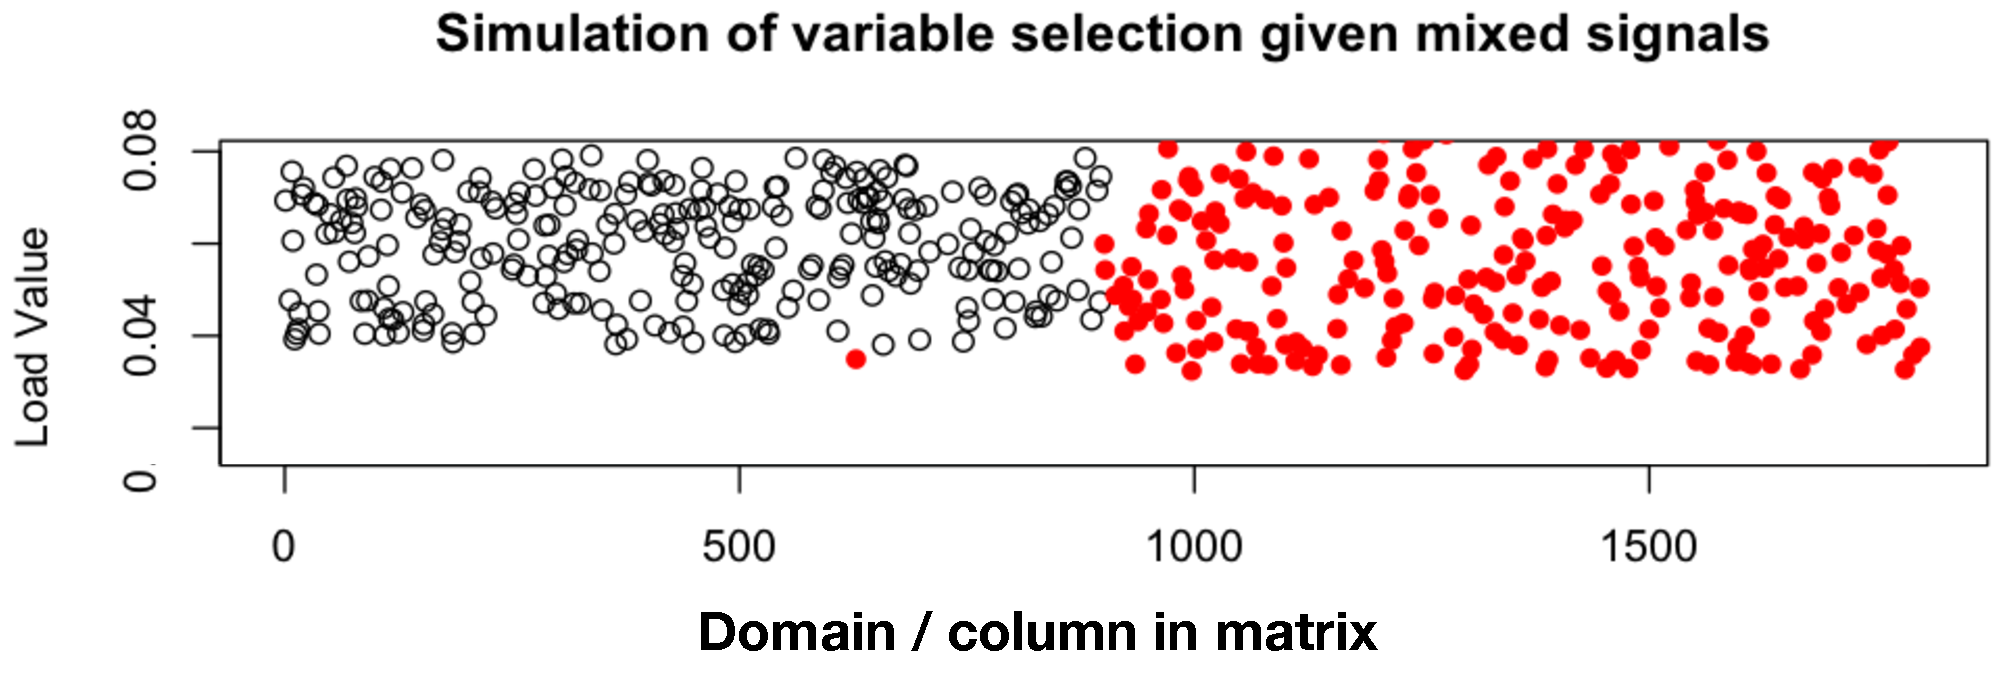
\includegraphics[width=120mm]{simulation_result_mix.pdf} 
\end{center}
\vspace{-0.2in}
\caption{The black hollow circles show the non-zero entries in
  $\bs\phi_{\X}$ that are selected by SCCA.  The red full circles show the non-zero entries in
  $\bs\phi_{\X}$ that are selected by PSCCA.  The $\Z$ signal factors
  out the confounding signal in the first half of the matrix leaving
  the second signal of interest in the second half to be the source of
the significant association.}
\end{figure}
\vspace{-0.1in}
% This analysis can be achieved by simulating imaging data and two other
% views (age, cognition) in such a way that the age is the true hidden variable that
% generates both cognition and imaging measurements.  PSCCA should then
% detect an insignificant association between cognition and imaging when
% age is used as the confounding variable.  Similarly, PSCCA should
% detect a significant association between age and imaging when
% cognition is a confounding variable.   
\subsection{Comparison of regression and PSCCA on OASIS data}
Our first evaluation on real data employs PSCCA as a form of
multivariate regression between imaging, diagnosis and nuisance variables.  
We employ a subset of the freely available OASIS dataset to compare
PSCCA to mass-univariate linear regression.  This subset of the OASIS
data contains elderly subjects (n=38) in addition to subjects with
Alzheimer's disease (n=31) of both genders (39 F, 30 M) and with ages
that range between 62 and 98 years.  Our evaluation criterion compares
both methods' power to detect the known anatomical distribution of
AD-related atrophy in gray matter (hippocampus, cuneus, temporal lobe)
\cite{Avants2010b} where gray matter was segmented and normalized by using standard
open source software.  We use the whole brain, in template space, as region of interest in order to
challenge the power of the mass-univariate method relative to the
single test performed by multivariate PSCCA.  We assume that the
researcher has pre-selected the sparseness parameter for the study.
We choose $\lambda$ (sparsity parameter) for the gray matter voxels such that 10\% of the
ROI (contained in the $\X$ matrix) will be selected by PSCCA.  The
$\Y$ matrix, in this case, is the diagnosis vector that defines
whether a subject is control or patient.  The nuisance matrix $\Z$
contains age and gender variables.  We run both the mass-univariate
statistics (via the {\bf R} program) and our own independently
developed PSCCA implementation (C++ based, BSD license, open-source)
on identical input data.  Using false discovery rate (FDR) correction
on the regression-based p-values for diagnosis, we find that the
minimum q-value is 0.183, thus insignificant after correction.  In
contrast, PSCCA shows significant effects at the $p=0.041$ level,
10000 permutations.  We visualize the regions that emerge from PSCCA
by overlaying the first canonical vector $\bs \psi_{\X}$ on the brain.
Figure~\ref{fig:comp} compares the PSCCA output with the regression
results overlaid on the brain at the level of $p=0.01$ uncorrected.
\vspace{-0.1in}
\begin{figure}
\label{fig:comp}
\begin{center}
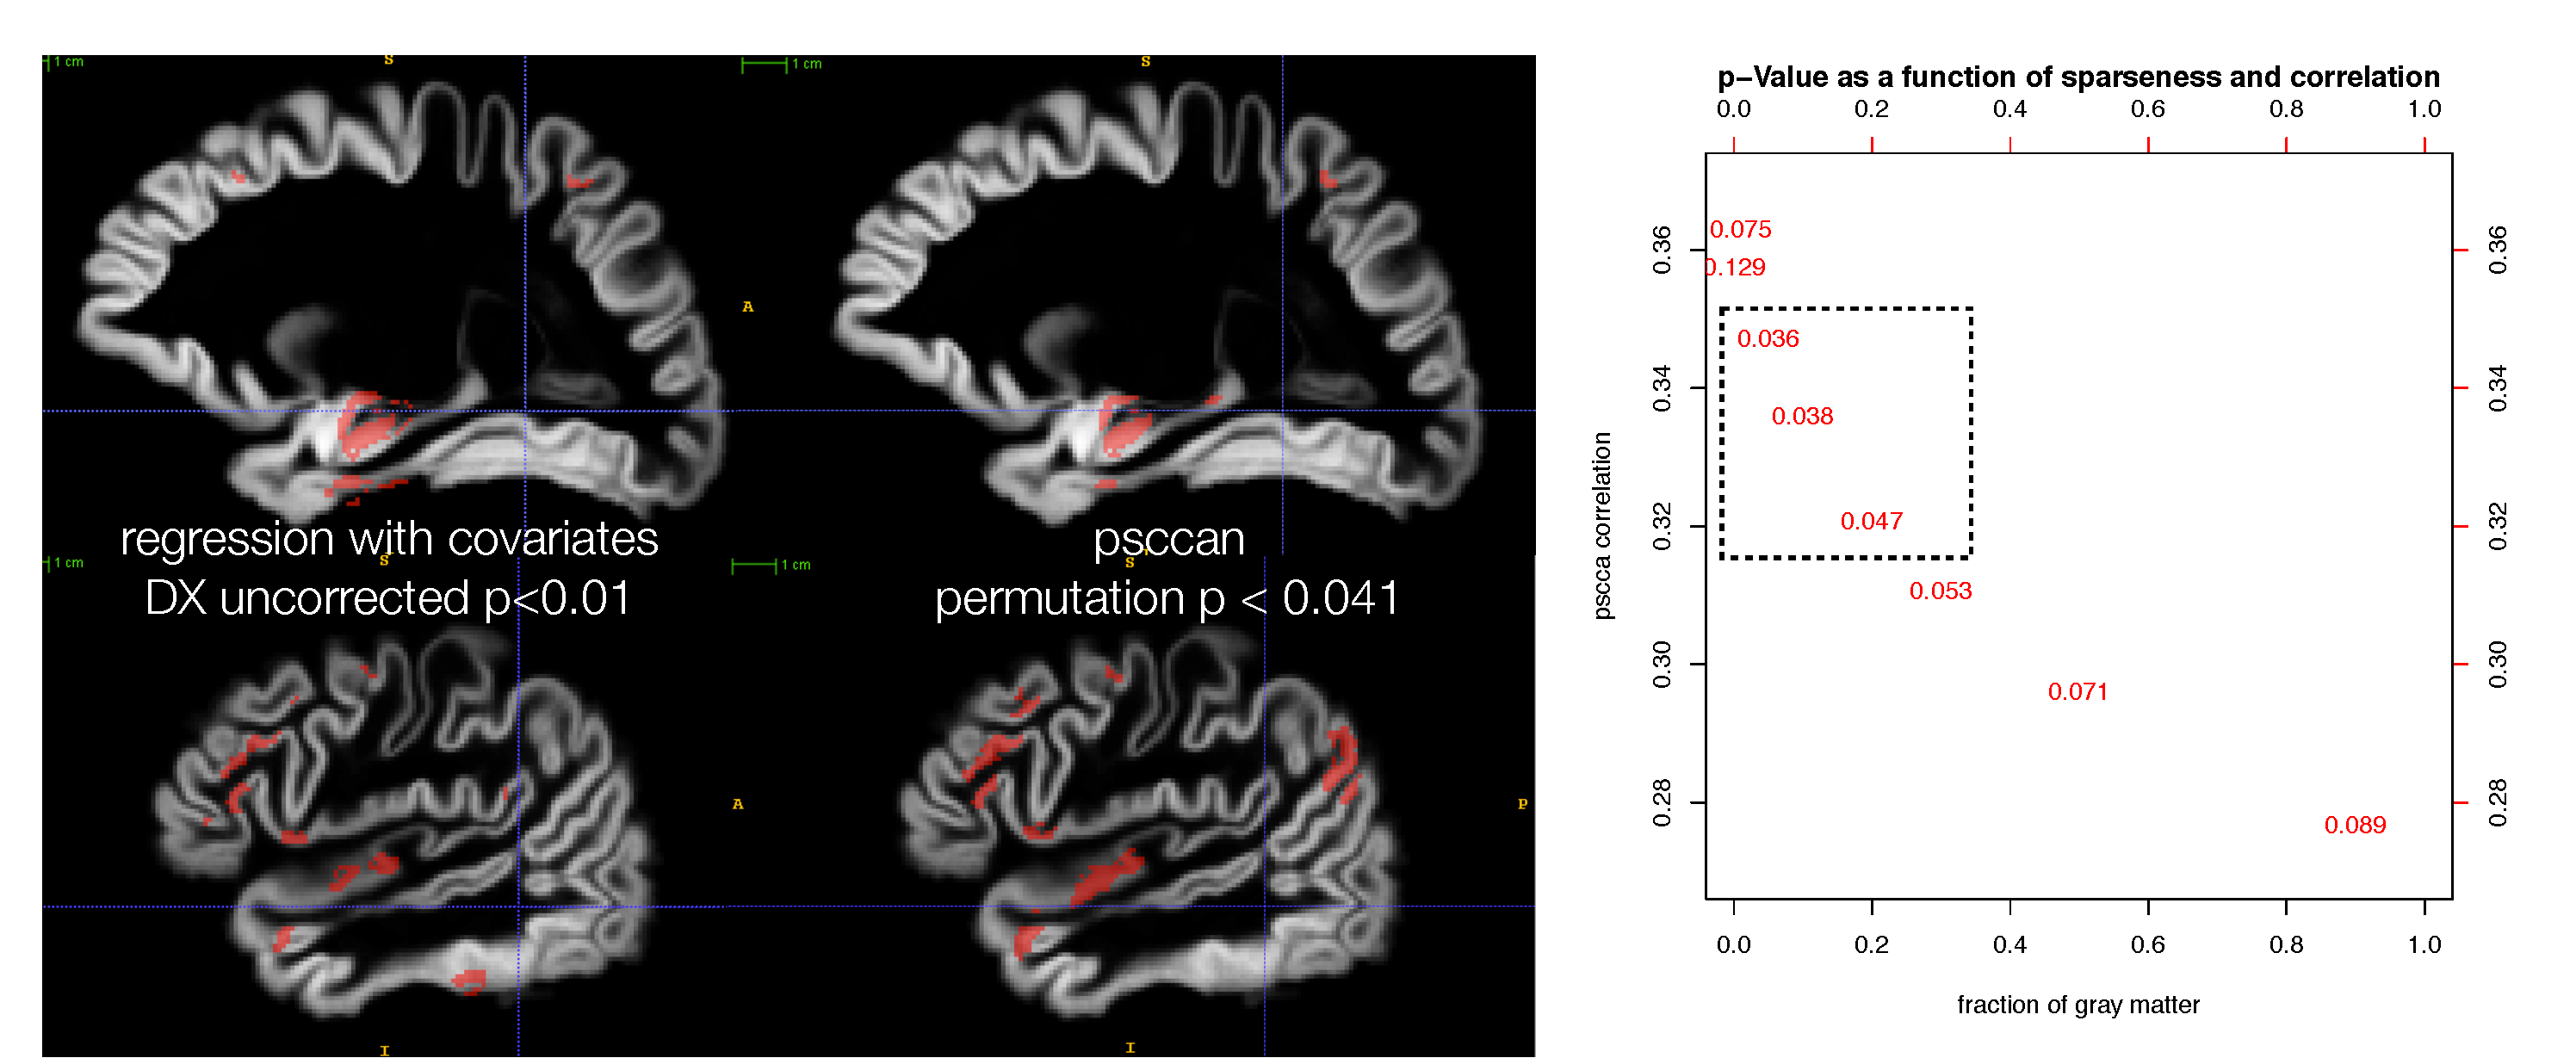
\includegraphics[width=120mm]{MUvPSCCAN.pdf} 
% \includegraphics[width=50mm]{Pvalue_f_of_sparsenss_and_corr.pdf} 
\end{center}
\vspace{-0.1in}
\caption{PSCCAN (right) versus mass-univariate uncorrected statistics
(left).  Both methods reveal similar areas of the brain.  However, the
mass-univariate results cannot be considered significant (after FDR
correction) due to the multiple comparisons problem.  It is possible
that another correction method would retain some of the mass-univariate
effects but we choose FDR because it is standard and only moderately
conservative.  We show, at right, the relationship of estimated
significance to variations in the sparseness parameter (for the image
voxel matrix $\X$) and PSCCA correlation.  The significant region is
outlined in a dashed box.  In a real study, one would only use the
pre-selected sparseness parameter.}
\end{figure}
\vspace{-0.1in}
\section{Discussion and Conclusion}
%\vspace{-0.1in}
In this paper we proposed a new statistical tool that is
ideal for multivariate imaging studies. 
% We presented the theory behind
% PSCCA and also provided a highly efficient algorithm for solving the
% optimization problem. Our formulation also has two user defined
% sparsity parameters $\lambda_{\X}$ and $\lambda_{\Y}$ which the
% researcher can chose based on domain knowledge or select automatically
% by optimizing on a held out development set. 
Results on synthetic and
real world data (OASIS) further corroborate our hypothesis that PSCCA
is able to increase detection power in the presence of covariates and
extract biologically plausible, multivariate patterns from neuroimaging
data.  Specifically, PSCCA reveals significant patterns of difference
between elderly and AD subjects that are within brain regions known to
be affected by Alzheimer's tauopathy.  Although the mass-univariate model fails to reveal
significant effects, there is notable similarity between regions selected by PSCCA and
those voxels in the brain that had uncorrected $p$-value $< 0.01$.  %This study has limitations.   
In our experiments we only use the
primary eigenvector from PSCCA;
Future work will analyze the effect of including additional
eigenvectors and will seek to further investigate alternatives for
assessing PSCCA significance in interpretable ways. Finally, as in standard correlation, one should take care to visualize PSCCA results to investigate the potential impact of outliers. 

% {\bf FINISH}
% despite the fact that we show similar biologically plausible patterns to univariate
% regression, though with greater power, 
% difficulty of interpretation remains ....  




%\noindent{\bf Acknowledgment}
% This work is supported by Grant XXX 
% 1R01EB006266-01 
% from the ...
%National Institute Of Biomedical Imaging and Bioengineering and administered through the UCLA Center for Computational Biology.
% %\vspace{-0.1in}
\bibliographystyle{IEEEbib}
\bibliography{./cca}

\end{document}


\text{argmax}( \x,\y) :
~\text{Corr}~( \X \x , \Y \y) - \lambda_\x \| \x \|_1 - \lambda_\y \|  \y  \|_1 , 
\end{equation} 
where $\X$ is a matrix with columns containing voxels from one set of
images of $n$ subjects, 
and $\Y$ is a matrix with columns containing voxels from the second
set of images from the same $n$ subjects. 
Corr computes Pearson correlation and the
$\lambda$ are inversely related to the sparseness costs, $C$.  %\vspace{-0.2in}

The covariance formulation of SCCA .... 

Let's compute the canonical correlation between two matrices where we
assume the matrices have been normalized and, as such, CCA computes
$$ \rho = \frac{ x \X^T \Y y  }{ \sqrt{x  \X^T \X x}\sqrt{x  \Y^T \Y y}  } $$.  Now, we change bases by
using the whitening transform.  
Redefine $\x =  ... $ Then, $\X \leftarrow \X \Sigma^{-1/2}_{XX}$ (same for $\Y$) and
$$ \rho = \frac{ x \X_w^T \Y_w \y  }{ ||x|| || y||} $$.
$$\rho = \frac{c^T \Sigma^{-1/2}_{XX} \Sigma_{XY}
  \Sigma^{-1/2}_{YY}}{\sqrt{c^Tc}\sqrt{d^Td}}$$

if matrices are whitened, then $\X \leftarrow \X \Sigma^{-1/2}_{XX}$
$$ \rho = \frac{c^T \Sigma_{XY}  d }{\sqrt{c^Tc}\sqrt{d^Td}}$$

The partial SCCA formulation will maximize 


Generally, SCCA depends upon univariate models to
factor out the effects of confounding variables.  In this paper we present a
novel algorithm for computing partial sparse canonical correlation
analysis (PSCCA) and factor (``partial'') out the effect of unwanted covariates. 

Sparse canonical correlation analysis (SCCA) is a powerful,
multivariate statistical tool for making unbiased inferences about the
relationship between different types of measurements taken on the same
population.
